% !TEX root =../prj4projektrapport.tex

\section{Indledning}

Formålet med dette projekt er at løse følgende problemformulering; \textit{Når belastningerne i et distributionssystem ændres, vil spændingsniveauet variere. Det er vigtigt, at spændingsniveauet holdes stabilt. Hvordan sikres dette?}
Udgangspunktet for problemstillingen er det lovmæssige krav, der siger, at spændingsforsyningen hos danske forbrugere altid skal ligge på 230 volt $\pm$10$\%$ \cite{Sikkerhedsstyrelsen}. Det ønskes at undersøge udfordringerne ved dette samt at komme med et bud på, hvordan denne problemstilling løses bedst muligt, både som elnettet ser ud i dag, men også i fremtiden. 

For at kunne arbejde med problemformuleringen og undersøge dens aktualitet, valgte projektgruppen at tage kontakt til energiselskabet Eniig. Det viste sig, at der på nuværende tidspunkt ikke foretages regulering på lavspændingsnettet, men i stedet på 60/10 kV transformere. Projektgruppen fandt det derfor interessant at undersøge mulighederne for regulering på lavspændingsnettet og eventuelle fordele og fremtidsaspekter ved dette.

I dette projekt vil fokus derfor være på den del af nettet, der går fra distributionstransformer og ud til forbrugere. For at sikre et stabilt spændingsniveau ønskes det at kunne overvåge tilstanden på distributionslinjen, ikke kun ved transformeren, men også ved hver enkelt forbruger. Det samlede system, der fremstilles i projektet betegnes som Spændingsregulator. Med denne ønskes det at lave et proof of concept i forhold til problemformuleringen. På grund af tilgængelighed af komponenter og udstyr vil prototypen for Spændingsregulator blive skaleret ned. 

For at belyse problemstillingen vil der i dette projekt blive lavet en simulering af en distributionslinje samt belastninger, der skal simulere forbrugere på linjen. Projektet vil desuden bestå af en trintransformer, der giver mulighed for at variere spændingsniveauet til linjen og forbrugerne på sekundærsiden af transformeren.

Til justering af spændingsniveauet, er det nødvendigt at kende til de aktuelle værdier for spændingen både centralt ved trintransformeren og decentralt ved forbrugerne. Af denne grund implementeres enheder til måling af spændingen. Det ønskes desuden at kende til systemets power factor, og derfor skal strømmen også måles. Et eventuelt indhold af harmoniske kan føre til unødig belastning og opvarmning af transformere, og det er derfor fornuftigt at kende til indholdet af harmoniske, og denne parameter skal også måles.
For at kunne holde et ønsket spændingsniveau vil der i projektet implementeres en enhed til regulering af trin på transformeren.

\begin{figure}[H]
	\centering
	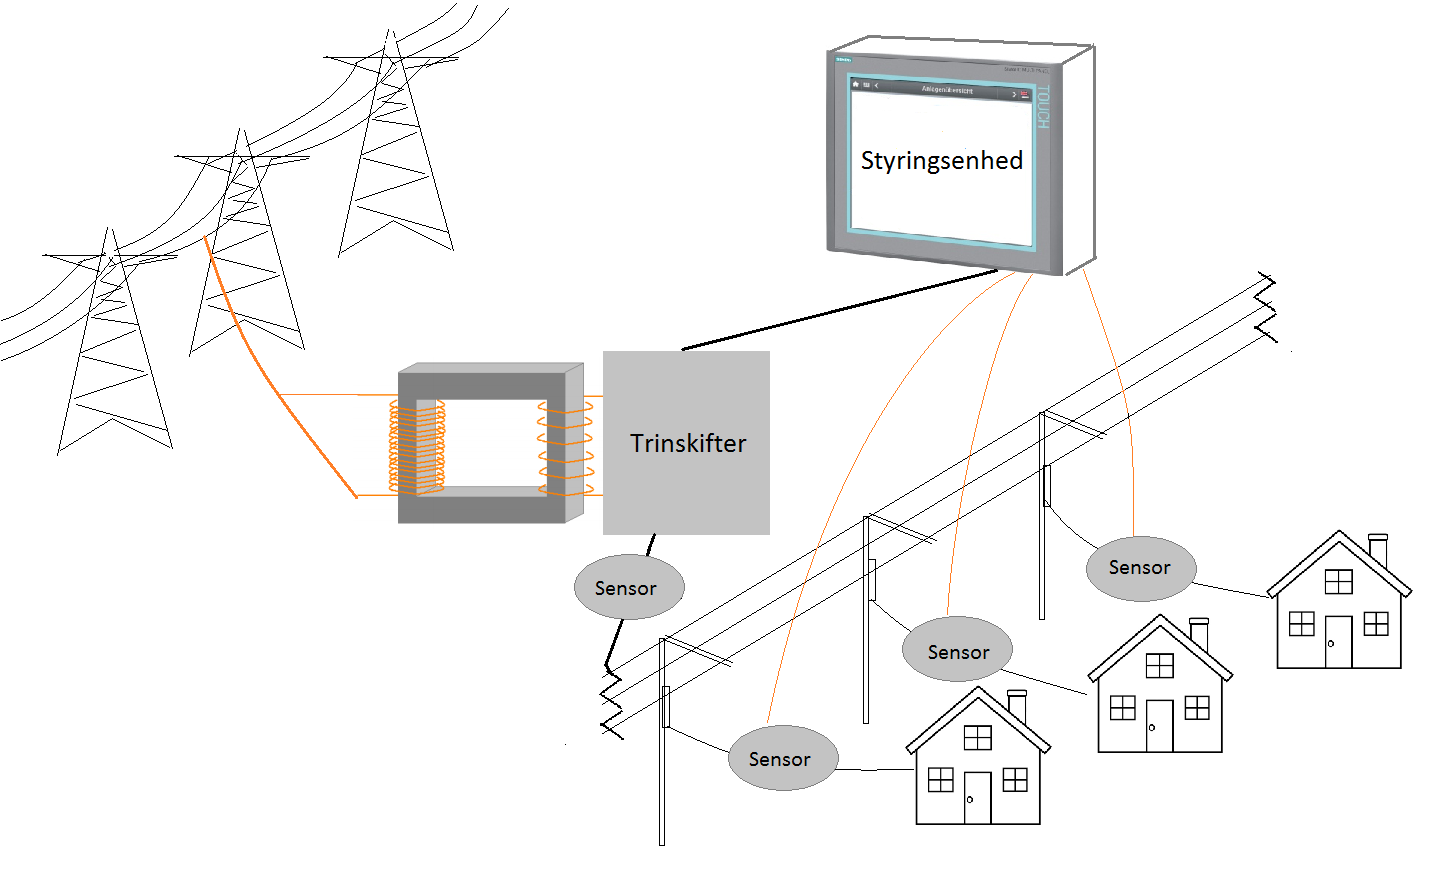
\includegraphics[width=1\textwidth]{figure/RigtBillede}
	\caption{Visuel fremstilling af Spændingsregulator}
	\label{fig:Rigtbillede}
\end{figure}

På figur \ref{fig:Rigtbillede} ses et rigt billede til at give oveblik over Spændingsregulatoren. Billedet viser trintransformeren, der forsyner distributionslinjen, Måleenheder, der måler aktuelle værdier på linjen og en Styringsenhed, der regulerer trintransformeren på baggrund af disse værdier. 